\chapter{Orientation Estimation}
\label{ch:orientation_estimation}

This chapter covers fundamentals of orientation estimation that are necessary for the implementation of the aforementioned system. In the motion monitoring field and especially in aircraft navigation the position of the coordinate frame of the body, with respect to a reference coordinate frame, is known as attitude, which is used as a synonym of orientation. There are different approaches to compute attitude estimates from magnetic and inertial data. This chapter explains their pros and cons and introduces sensor fusion as a means to mitigate the drawbacks of each approach. Beforehand, two main mathematical constructs used to express attitude -- Euler angles and quaternions -- are described.

\section{Euler Angles}

Euler angles are one of several ways to describe the orientation of an object and its associated body frame in three-dimensional Euclidean space, with respect to a reference frame. They represent a sequence of three elemental rotations about the axes of the coordinate system, defined as follows:

\begin{itemize}
\item The \emph{roll} angle $\phi$ determines the rotation around the $x$-axis.
\item The \emph{pitch} angle $\theta$ determines the rotation around the $y$-axis.
\item The \emph{yaw} angle $\psi$ determines the rotation around the $z$-axis.
\end{itemize}

\noindent
Figure \ref{fig:Euler_angles} depicts the rotation about the axes $z, y', X$ by $\psi, \theta, \phi$, respectively, according to the Tait-Bryan convention. The colour blue indicates the orientation before and the colour red the orientation after the rotation. In contrast to extrinsic rotations, where the three elemental rotations may occur either about the axes of the original coordinate system, the Tait-Bryan rotations are intrinsic rotations that occur about the axes of the rotating coordinate system, which changes its orientation after each rotation.

\begin{figure}
\centering
\begin{tikzpicture}[scale=1.4]
\node[inner sep=0pt] (tait) at (0,0)
    {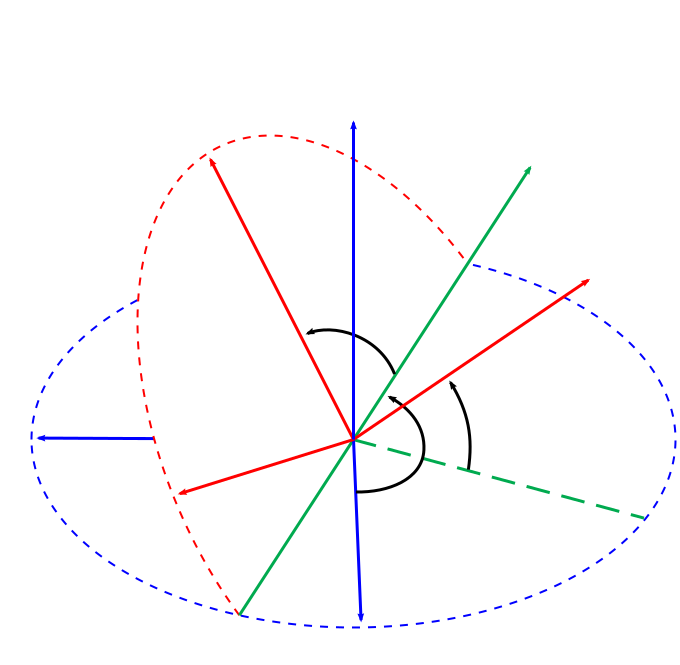
\includegraphics[width=.7\textwidth]{Images/taitbryan.pdf}};
    
\node [] at (0.5,0.2) {$\phi$};
\node [] at (0.65,-1.85) {$\psi$};
\node [] at (1.55,-0.9) {$\theta$};

\node [] at (-3.4,-1.1) {$x$};
\node [] at (0.25,-3.3) {$y$};
\node [] at (0.12,2.43) {$z$};

\node [] at (2.8,0.6) {$X$};
\node [] at (-1.5,2.05) {$Y$};
\node [] at (-2.0,-1.7) {$Z$};
\end{tikzpicture}
\caption{Representation of the body frame (red) with respect to the navigation frame (blue). The body frame was rotated, by the Euler angles $\psi, \theta, \phi$ about the axes $z, y', X$, respectively. Adapted from \cite{Wiki_taitbryan}.} \label{fig:Euler_angles}
\end{figure}

Euler angles are a simple and intuitive means to represent rotations in three-dimensional space. However, for the above mentioned parameterisation they have singularities at values of $\theta = n \pi$, $n \in \mathbb{Z}$. At these points a rotation about the $x$-axis and the $z$-axis constitute the same motion, which results in the loss of one degree of freedom and makes changes in $\phi$ and $\psi$ indistinguishable. This phenomenon is called \emph{gimbal lock}. The usage of \emph{quaternions} instead of Euler angles avoids the problem of gimbal locks.

\subsection{Transformation Matrix}

Coordinates representing a point in one coordinate system can be transformed to another. Such a transformations can be expressed as multiplication of a matrix with the coordinate vector that is to be transformed. Let $\mathbf{E}$ denote the orthonormal basis $\{x, y, z\} \in \mathbb{R}^3$ and let $\mathbf{E}'$ denote the orthonormal basis $\{X, Y, Z\} \in \mathbb{R}^3$. Furthermore, let $\mathbf{p}$ denote the position vector of an arbitrary point in three-dimensional Euclidean space. The coordinate transformation from $\mathbf{E}$ to $\mathbf{E}'$ is denoted $\bm{\Omega}_{\mathbf{E} \rightarrow \mathbf{E}'}: (p_1, p_2, p_3) \mapsto (p'_1, p'_2, p'_3)$. Then, the linear transformation from $\mathbf{p}$ to $\mathbf{p}'$ is given by

\begin{equation}\label{eq:transformation}
  \mathbf{p'} = \bm{\Omega}_{\mathbf{E} \rightarrow \mathbf{E}'}(\mathbf{p}) = \mathbf{T} \mathbf{p}\,,
\end{equation}

\noindent
where $\mathbf{T}$ is the transformation matrix.

To transform the coordinate vector from the navigation frame to the body frame, according to the common aerospace rotation sequence mentioned above and the Nort-East-Down system (NED), the transformation matrix $\mathbf{C}_{nb}$ is given by

\begin{equation}\label{eq:transformation_matrices}
\begin{split}
\mathbf{C}_{nb} & = \mathbf{T}_x(\phi) \mathbf{T}_y(\theta) \mathbf{T}_z(\psi) \\
 & = {\left[ \begin{smallmatrix}
    1 \; & 0 \; & 0 \\
    0 \; & \cos \phi \; & \sin \phi \\
    0 \; & -\sin \phi \; & \cos \phi
    \end{smallmatrix}\right]}
    {\bigg[ \begin{smallmatrix}
    \cos \theta \; & 0 \; & -\sin \theta \\
    0 \; & 1 \; & 0 \\
    \sin \theta \; & 0 \; & \cos \theta
    \end{smallmatrix} \bigg]}
    {\left[\begin{smallmatrix}
    \cos \psi \; & \sin \psi \; & 0 \\
    -\sin \psi \; & \cos \psi \; & 0 \\
    0 \; & 0 \; & 1
    \end{smallmatrix}\right]}\\
 & = {\left[\begin{smallmatrix}
   \cos \theta \cos \psi \; &
    \cos \theta \sin \psi \; &
   -\sin \theta \\
    \sin \phi \sin \theta \cos \psi - \cos \phi \sin \psi \;\; &
    \sin \phi \sin \theta \sin \psi + \cos \phi \cos \psi \;\; &
    \sin \phi \cos \theta \\
    \cos \phi \sin \theta \cos \psi + \sin \phi \sin \psi \;\; &
    \cos \phi \sin \theta \sin \psi - \sin \phi \cos \psi \;\; &
    \cos \phi \cos \theta
  \end{smallmatrix}\right]}
\end{split}
\end{equation}

\noindent
Plugged in Equation \ref{eq:transformation} ($\mathbf{T} = \mathbf{C}_{nb}$) the left multiplications of the matrices $\mathbf{T}_x(\phi), \mathbf{T}_y(\theta), \mathbf{T}_z(\psi)$ to the vector $\mathbf{p}$ represent the coordinate rotations about the single axes $x, y, z$, respectively. That is, the orthogonal projection onto the axes of the coordinate system, which result from the respective two-dimensional rotation of $\phi, \theta, \psi$ about the axes $x, y, z$, is computed. This is illustrated for a single rotation around the $z$-axis by the angle $\psi$ in Figure \ref{fig:transformation_matrix}. The matrices $\mathbf{T}_x(\phi), \mathbf{T}_y(\theta)$, and $\mathbf{T}_z(\psi)$ are also known as direction cosine matrices, since their elements are the cosines of the unsigned angles between the body-fixed axes and the axes of the navigation frame, as shown in \cite{diebel2006attitude}. The form stated here is already simplified. The matrix $\mathbf{C}_{bn}$ for transforming the coordinate vector from the body frame to the navigation frame is given by

\begin{figure}
\centering

\tdplotsetmaincoords{60}{110}

\begin{tikzpicture}[scale=6,tdplot_main_coords]

\coordinate (O) at (0,0,0);
\pgfmathsetmacro{\psivec}{55}
\tdplotsetcoord{P}{0.8}{44}{\psivec}

\draw[thick,->] (0,0,0) -- (.8,0,0) node[anchor=north west]{$x$};
\draw[thick,->] (0,0,0) -- (0,.8,0) node[anchor=north west]{$y$};

\tdplotsetrotatedcoords{0}{0}{25}

\draw[thick,blue,tdplot_rotated_coords,->] (0,0,0) -- (.8,0,0) node[anchor=north west]{$x'$};
\draw[thick,blue,tdplot_rotated_coords,->] (0,0,0) -- (0,.8,0) node[anchor=west]{$y'$};
\draw[very thick,blue,tdplot_rotated_coords] (0,0,0) -- (0, 0.25, 0) node[anchor=south east]{$p_y'$};
\draw[thick,blue,tdplot_rotated_coords,->] (0,0,0) -- (0,0,.8) node[anchor=north west]{$z'=z$};
\draw[very thick,blue,tdplot_rotated_coords] (0,0,0) -- (0.507, 0, 0) node[pos=0.9, label={left:$p_x'$}, rounded corners=1pt]{};
\draw[very thick,blue,tdplot_rotated_coords] (0,0,0) -- (Pz) node[pos=0.5, label={left:$p_z'$}]{};

%draw a vector from origin to point (P) 
\draw[-stealth,color=red] (O) -- node [anchor=south]{$p$}(P);

%draw projection on xy plane, and a connecting line
\draw[dashed, red] (O) -- (Pxy);
\draw[dashed, red] (P) -- (Pxy);
\draw[dashed] (Px) -- (Pxy);
\draw[dashed] (Py) -- (Pxy);

\tdplotdrawarc[-stealth]{(0,0,0)}{0.58}{0}{25}{anchor=north}{$\psi$}

\draw[dashed] (0.8,0,0) arc (0:115:0.8);

\draw[dashed, blue, tdplot_rotated_coords] (0.507, 0, 0) -- (Pxy);
\draw[dashed, blue, tdplot_rotated_coords] (0, 0.25, 0) -- (Pxy);
\draw[dashed, blue, tdplot_rotated_coords] (P) -- (Pz);

\end{tikzpicture}
\caption{An exemplary coordinate rotation about the $z$-axis by an angle $\psi$, illustrating the orthogonal projection on the resulting axes $x', y', z'$.}
	\label{fig:transformation_matrix}
\end{figure}


\begin{equation}
\mathbf{C}_{bn} = {\left[\begin{smallmatrix}
   \cos \theta \cos \psi \; &
    \sin \phi \sin \theta \cos \psi - \cos \phi \sin \psi \; &
    \cos \phi \sin \theta \cos \psi + \sin \phi \sin \psi \\
    \cos \theta \sin \psi \;\; &
    \sin \phi \sin \theta \sin \psi + \cos \phi \cos \psi \;\; &
    \cos \phi \sin \theta \sin \psi - \sin \phi \cos \psi \\
    -\sin \theta \;\; &
    \sin \phi \cos \theta \;\; &
    \cos \phi \cos \theta
  \end{smallmatrix}\right]}
\end{equation}

\noindent
Note that $\mathbf{C}_{bn} = \mathbf{C}^T_{nb} = \mathbf{C}^{-1}_{nb}$. Thus, $\mathbf{C}^{ }_{bn}$ and $\mathbf{C}_{nb}$ are orthogonal matrices so that $\mathbf{C}^{ }_{bn} \mathbf{C}_{nb} = \mathbf{I}$.  

\section{Quaternions}

Quaternions are a number system that extends the complex numbers. They were first described by Irish mathematician William Rowan Hamilton in 1843. The set of quaternions is equal to $\mathbb{R}^4$ and denoted with $\mathbb{H}$. A quaternion $\mathbf{q} \in \mathbb{H}$ may be represented as

\begin{equation}
  \mathbf{q} = q_0 + q_1 i + q_2 j + q_3 k = \begin{bmatrix}
  	q_0, & q_1, & q_2, & q_3
  \end{bmatrix}^T = \begin{bmatrix}
  	q_0 \\ \mathbf{q}_{1:3} 
  \end{bmatrix}\,,
\end{equation}
 
\noindent
whereby the following relations between the imaginary units $i, j, k$ hold:

\begin{equation}
  \begin{matrix}
i^2 =j^2=k^2=ijk =-1\,,\\ \\
  {\begin{split}
  ij & = k, \qquad ji = -k, \\
jk & = i, \qquad kj = -i, \\
ki & = j, \qquad ik = -j\,.
\end{split}}
\end{matrix}
\end{equation}

The \emph{adjoint}, \emph{norm} and \emph{inverse} of a quaternion are defined as

\begin{equation}
  \bar{\mathbf{q}} = \begin{bmatrix}
  	q_0 \\ -\mathbf{q}_{1:3} 
  \end{bmatrix}\,,
\end{equation}

\begin{equation}
  ||\mathbf{q}|| = \sqrt[]{q_0^2 + q_1^2 + q_2^2 + q_3^2}
\end{equation}

\begin{equation}
	\mathbf{q}^{-1} = \frac{\bar{\mathbf{q}}}{||\mathbf{q}||}
\end{equation}

The sum of two quaternions is defined as

\begin{equation}
  \mathbf{q} + \mathbf{p} = \begin{bmatrix}
  	q_0 + p_0 \\ \mathbf{q}_{1:3} + \mathbf{p}_{1:3}
  \end{bmatrix}\,.
\end{equation}

Quaternion multiplication is defined as

\begin{equation}
  \mathbf{q} \mathbf{p} = \begin{bmatrix}
  	q_0 p_0 -\mathbf{q}^T_{1:3} \mathbf{p}_{1:3}\\
  	q_0 \mathbf{p}_{1:3} + p_0 \mathbf{q}_{1:3} - \mathbf{q}_{1:3} \times \mathbf{p}_{1:3}
  \end{bmatrix}\,,
\end{equation}

\noindent
and can be written as the second quaternion left-multiplied by a matrix-valued function $Q$ of the first quaternion.

\begin{equation}
  \mathbf{q} \mathbf{p} = Q(\mathbf{q}) \mathbf{p} = \bar{Q}(\mathbf{p}) \mathbf{q}
\end{equation}

\noindent
The \emph{quaternion matrix function}, $Q : \mathbb{H} \rightarrow \mathbb{R}^{4\times4}$ is defined by

\begin{equation}
	Q(\mathbf{q}) = \begin{bmatrix}
 q_0 & -q_1 & -q_2 & -q_3\\
 q_1 & q_0 & q_3 & -q_2\\
 q_2 & -q_3 & q_0 & q_1 \\
 q_3 & q_2 & -q_1 & q_0
\end{bmatrix}\,,
\end{equation}

\noindent
and the \emph{conjugate quaternion matrix function}, $\bar{Q} : \mathbb{H} \rightarrow \mathbb{R}^{4\times4}$ is defined by

\begin{equation}
	\bar{Q}(\mathbf{q}) = \begin{bmatrix}
 q_0 & -q_1 & -q_2 & -q_3\\
 q_1 & q_0 & -q_3 & q_2\\
 q_2 & q_3 & q_0 & -q_1 \\
 q_3 & -q_2 & q_1 & q_0
\end{bmatrix}\,.
\end{equation}



Unit quaternions, i.\,e. quaternions with unity norm, can be used to represent rotations in three dimensional space. Let $\mathbf{z} \in \mathbb{R}^3$ be an arbitrary vector in the navigation frame and let $\mathbf{z}' \in \mathbb{R}^3$ be the same vector in the body frame. Furthermore, let $\mathbf{r}$ be a quaternion with $||\mathbf{r}|| = 1$. Then the following relations hold:

\begin{equation}
  \begin{bmatrix}
  	0 \\ \mathbf{z}' 
  \end{bmatrix} = \mathbf{r} \begin{bmatrix}
  	0 \\ \mathbf{z} 
  \end{bmatrix} \mathbf{r}^{-1}\,,
\end{equation}

\begin{equation}
  \begin{bmatrix}
  	0 \\ \mathbf{z} 
  \end{bmatrix} = \mathbf{r}^{-1} \begin{bmatrix}
  	0 \\ \mathbf{z}' 
  \end{bmatrix} \mathbf{r}\,.
\end{equation}

\noindent
Sequences of rotations can thus be represented by products of quaternions. The quaternion for a single rotation by $\alpha$ about the axis $\bm{\epsilon} \in \mathbb{R}^3$, $||\bm{\epsilon}|| = 1$, is given by

\begin{equation}
\begin{split}
  \mathbf{r}_{\epsilon}(\alpha, \bm{\epsilon}) &= \begin{bmatrix}
  	\cos \frac{\alpha}{2}, & \bm{\epsilon} \sin \frac{\alpha}{2}
  \end{bmatrix}^T \\
  &= \begin{bmatrix}
  	\cos \frac{\alpha}{2}, & \epsilon _1 \sin \frac{\alpha}{2}, & \epsilon _2 \sin \frac{\alpha}{2}, & \epsilon _3 \sin \frac{\alpha}{2}
  \end{bmatrix}^T\,.
\end{split}
\end{equation}

\noindent
The reverse mapping from quaternions to Euler angles is given by

\begin{equation}
  \begin{bmatrix}
\phi \\ \theta \\ \psi
\end{bmatrix} =
\begin{bmatrix}
\mbox{atan}2 ((2(q_0 q_1 + q_2 q_3), 1 - 2(q_1^2 + q_2^2)) \\
\mbox{arcsin} (2(q_0 q_2 - q_1 q_3)) \\
\mbox{atan}2 (2(q_0 q_3 + q_1 q_2), 1 - 2(q_2^2 + q_3^2))
\end{bmatrix}\,.
\end{equation}

Quaternions are less intuitive than Euler angles. Nevertheless, they are very popular in attitude representation, since they are mathematically elegant and don't suffer from singularities.

\section{Projection of the Gravity Vector and Earth's Magnetic Field Vector}

As described in Chapter \ref{ch:MARG}, accelerometers measure the linear acceleration they experience. Under static or quasi-static (steady, linear motion) conditions, or at low acceleration it can be assumed that the measured acceleration is mainly that of gravity. Be means of simple trigonometric functions estimates for the pitch and the roll angle can be obtained. Since the gravity vector is perpendicular to the $xy$-plane and thus a rotation around the $z$-axis will not cause any variation in the sensed acceleration, the yaw angle cannot be obtained by this method. To solve this problem a three-dimensional magnetometer is used, which measures the variation of Earth's magnetic field while rotating around the $z$-axis.

When the accelerometer is motionless, its measurements will be directly related to the angle of the sensor relative to gravity, as depicted in Figure \ref{fig:acceleration_motion} (a). In that case $\theta$ is given by

\begin{equation} \label{eq:projection_gravity}
  \theta = \mbox{atan}2(A_y, A_x)\,.
\end{equation}

\noindent
However, when the sensor is in motion, in addition to the gravity, there are radial and tangential acceleration components due to motion, as depicted in Figure \ref{fig:acceleration_motion} (b). Ignoring these components will cause incorrect angle estimates.

\begin{figure}
\centering
\begin{subfigure}[]{0.45\textwidth}
\caption{}
\begin{tikzpicture}[auto, thick, node distance=3cm,>=latex']
    \node [draw, very thick, rounded corners=1pt, rectangle, minimum height=6em, minimum width=3em, align=center, rotate around={27:(-1,0.5)}] (sensor) {Sensor};
    \node[coordinate] (A) at (0.7, -0.6) {};
    \node[coordinate] (B) at (1.95, -3) {};
    \node[coordinate] (C) at (0.7, -3.56) {};
    
    \draw[->] (A) -- node[name=x] {$A_x = g \cos \theta$}(B);
    \draw[->] (B) -- node[name=y] {$A_y = g \sin \theta$}(C);
    \draw[->, very thick] (A) -- node[name=g, label={left:$g$}] {}node [pos=0.35]{$\theta$} (C);
  
 	\draw (0.7,-2.0) arc (270:297:1.4);
      
    \end{tikzpicture}
\end{subfigure}
\quad
\begin{subfigure}[]{0.45\textwidth}
\caption{}
\begin{tikzpicture}[auto, thick, rounded corners=1pt, node distance=3cm,>=latex']
    \node [draw, very thick, rectangle, minimum height=6em, minimum width=3em, align=center, rotate around={27:(-1,0.5)}] (sensor) {Sensor};
    \node[coordinate] (A) at (0.7, -0.6) {};
    \node[coordinate] (B) at (2.1, -3.55) {};
    \node[coordinate] (C) at (0.7, -3.56) {};
    \node[coordinate] (D) at (1.2, -4) {};
    
    \draw[->, red, very thick] (A) -- node[name=d] {} (D);
    \draw[->] (A) -- node[name=x] {$A_x = A_{rad} + g \cos \theta$} node [pos=0.46, label={left:$\theta$}]{} (B);
    \draw[->] (B) -- node[name=y] {$A_y = A_{tan} + g \sin \theta$} (D);
    \draw[->, very thick] (A) -- node[name=g, label={left:$g$}] {}(C);
      
    \draw (0.953,-2.2) arc (270:304:0.8);  
      
    \end{tikzpicture}	
\end{subfigure}

\caption{Acceleration seen by the sensor (b) with and (a) without motion, from \cite{bennett_motion_2014}.} \label{fig:acceleration_motion}
\end{figure} 

\section{Integration of Angular Rate}

Another way to estimate the attitude of an object is the integration of the angular rate around the $x, y$ and $z$-axis, respectively. Although this would theoretically lead to very accurate orientation estimates, they are impaired by \gls{ARW} and dynamical bias in practice. \gls{ARW} is an effect caused by the integration of high-frequency, thermo-mechanical noise, which leads to a random additive angle in the orientation signal. An even greater impact than AWR has the gyroscopes dynamic bias, which has its origin in low-frequency flicker noise. Both effects cause a dramatical drift in the angle signal over time.

\section{Sensor Fusion}

Since the projection of the gravity vector is only valid under static or quasi-static conditions, or at low acceleration, and the integration of the angular rate leads to non-reliable estimates due to \gls{ARW} and dynamic bias, but is not affected by the intensity of motion, a means to combine the information of both sensors is desirable. The combination of information from multiple sensors to increase the overall precision of the estimation of a certain quantity of interest is termed \emph{sensor fusion}. \citeauthor{raol2009multi} \cite{raol2009multi} states the following advantages of sensor fusion:
 
\begin{itemize}
\item Robust functional and operational performance is given, in case of data loss from one sensor, due to redundancy provided by multiple sensors.
\item Enhanced confidence in the results inferred from the measurement of one sensor, if they are confirmed by the measurement of another sensor.
\item With sensor fusion an arbitrary fine time resolution of measurements is possible, whereas single sensors need a finite time to transmit measurements and so limit the frequency of measurements.
\item One sensor might be, to some extent, better in a certain state of the measured process, e.g. low or high motion intensity in attitude estimation, and thus, by fusing multiple sensor signals, a satisfactory accuracy among all states of the process could be attained.
\end{itemize}

\noindent
Sensor fusion can be realised by the use of a Kalman filter, which is described in detail in the next chapter.


